\documentclass[a4paper,11pt,titlepage]{article}
\usepackage[margin=25mm]{geometry}
\usepackage[T1]{fontenc}
\usepackage[utf8]{inputenc}
\usepackage{graphicx, wrapfig, subcaption}
\usepackage{mathtools}
\usepackage{url}
\usepackage{parskip}
\usepackage{pdfpages}
\usepackage{multicol}
\usepackage{multirow}
\usepackage{setspace}
\usepackage[bottom]{footmisc}
\setstretch{1.15}

\bibliographystyle{plain}

%\title{Bachelor Project}
%\begin{titlepage}
\title{Department of Mathematical Sciences \\
\vspace{0.5cm}
Bachelor Project \\
\vspace{1cm}
\Huge  Predictive Analysis of an Attribute Modelled by a Random Field % kanskje skrive tittel på oppgave? 
}
\author{\Large Filip Schjerven}
\date{\Large \today}
%\pagenumbering{none}
%\end{titlepage}
\begin{document}
\maketitle

\newpage
\section*{Summary}
%Oppsummering av hele oppgaven, problemstilling, metode, resultat/konklusjon
%MAX 1 side
\pagenumbering{roman}
\newpage
\pagenumbering{arabic}
\addcontentsline{toc}{section}{Summary}
\tableofcontents
\newpage
\listoffigures

\newpage

\section{Introduction}
%Skriv en innledning, hva handler oppgaven om (tema, problemstilling, hensikten:hva er det du vil finne ut), hva var motivasjonen for den

This report is written in coherence with the bachelor project for my studies within the Department of Mathematical Sciences at NTNU. The overall focus of this project is a case that will be handled with tools from spatial statistics. 

Spatial statistics refers to the application of statistical methods in a spatial setting. Statistics in itself is an extremely useful mathematical tool to quantify uncertainty. Uncertainty is something that we all face in a day to day basis in our daily lives, but perhaps even more so when viewing the world through scientific research. How can we know that our measurements, and thus how the world is described, are certain? In this sense, Cressie \& Wikle refers to statistics as the "Science of Uncertainty". Statistics has many ways of dealing with uncertainty, and one of them is that is interprets uncertainty as a measure of \textit{variability}. Other interpretations could also be used, like \textit{entropy}. By modelling uncertainty via variability, one may model the total variability by the variability in measurements, the model used and due to the uncertainty of parameters in the model \cite{CressieEtAl}. All this happens with the focus on acquiring information from the data that are to be modelled. In spatial statistics, all this happens in a spatial setting, i.e. the data that are to be analyzed via their topological, geometric or geographic attributes.

A typical model thats used in spatial statistics is a \textit{Gaussian Random Field} (GRF). Informally, a GRF is a collection of data that have been given a multivariate Gaussian joint probability function. The random field that it is 'attached' to typically defines the relation between the variables in some quantifiable way. A typical example (that will also be used extensively) is spatial location. As the joint probability function is multivariate Gaussian, all subsets of variables that are included in the GRF is also multivariate Gaussian with their attributes still defined by the relation inherited from the GRF. Due to the many useful properties of a multivariate Gaussian distributed variable, the GRF is a useful way to model data. 

In order to model data in a easy to interpret way, a model for GRF is often used to describe the various parts of the model. An example that wil be used in this project is the \textit{Bayes hierarchical model} (BHM). The exact formulation of a BHM is presented later, but summarized it consists of a 1) data model for specifying the data acquirement, 2) a process model for describing the latent process that is typically of interest and lastly any parameter-priors that are used in the Bayesian setting in 3) prior model. By distinguishing between the three, interpretability is made easy and one gets an intuitive way to understand the data acquirement how it relates to the latent process that is often of interest. 

As the latent process is of interest, making the correct data acquirement is crucial in order to achieve sufficient information from the data. In spatial statistics this is important, as the data must then be sampled at the correct locations. A set of measurement-locations is called a \textit{sampling design}, or simply \textit{design}, in spatial setting. Choosing the correct sampling design may be crucial for achieving the desired information, and must be evaluated with possible limitations as cost and precision of measurements. Constructing sampling designs happens typically in two settings, \textit{retroactive design} and \textit{proactive design}. A retrospective design will focus on altering the existing design on the basis of new data, while a proactive design will focus on constructing the optimal design on the basis of prior and estimated posterior data. 

This paper is organized into 5 sections, including the introduction and conclusion. Section 2 introduces the GRF by going through some basics and relevant properties of random fields, covariance functions and Gaussian processes. A short summary of \textit{Generalized Least Squares} (GLS) and hierarchical models is also part of this section, as it is to be used in the case scenario. The posterior distribution needed for the case scenario in section 4 is also derived. Section 3 introduces the notion of spatial sample design and how it may be related to the model in a quantifiable way. Some examples of path planning criterias is presented along with a short summary of the situation it were used in. Section 4 presents a case that the theory of section 2 and 3 will be applied upon. Input for the case and chosen modelspecification is presented, along with some case-specific procedures for estimating parameters based on the input data. Results follow in the last subsection of section 4, before the conclusion round up the main points of this paper.  

\subsection*{Notation} 
Throughout this text I'll refer to 
\newpage
\section{Spatial Gaussian Random Fields}
\subsection{Random Fields}
\textbf{Dette stykket om random fields må vel forbedres}

A random field is a set of random variables $\vec{Y}$ that has a distribution function 
\begin{equation} \label{eq:distribution_function}
F(Y(s_1) \leq y_1, \dots , Y(s_n) \leq y_n)
\end{equation} 

for any number $n$. A random field has typically some attribute that connects the random variables in $\vec{Y}$. Some examples of such attributes may be physical location, placement in a graph or ordering in time.

Depending on the properties of the distribution function and the setting in which it is defined, we have many different types of random fields, e.g. Markov Random Fields, Gibbs Random Fields and Conditional Random Fields, all of which may again be used with different attributes connecting the variables of the field. 

For this particular project, the main focus will revolve around a random field of type \textit{Gaussian Random Field} (GRF). A GRF is set up so that the variables $\vec{Y}$ is governed by a \textit{Gaussian process}. In addition, the Gaussian process will be assumed to be time-stationary, meaning that the Gaussian probability distributions of the process is invariant to changes in time. The variance of the process will be equal over the whole field, meaning that its spatially stationary as well. 

\subsection{Covariance functions} \label{sec:covariance_functions}

For a GRF with equal variance for all associated variables, two of them being $X$ and $Y$, we have that the covariance is defined by:
\begin{align*}
\frac{Cov( X, Y )}{\sqrt{Var( X )}\sqrt{Var( Y )}} = \frac{Cov( X, Y )}{\sigma^2} &= Corr(X, Y) \\
\implies  Cov( X, Y ) &= \sigma^2 Corr(X, Y)
\end{align*}
with $\sigma^2$ being the variance parameter of the covariance function. So the covariance of two variables are linear their pairwise correlation. \\

Evidently, by defining a covariance function to use for a Gaussian process, one achieves a expression covariance with fewer parameters to estimate or set. This simplification is desireable and acceptable for many different models, as we now are down to estimate or set what is typically a couple of parameters compared to estimating $\frac{(n-1)\cdot(n - 2)}{2}$ covariances for a Gaussian process with $n$ variables. In addition, by using a defined covariance function one is then guaranteed that the resulting covariance matrix is a \textit{positive definite matrix} \footnote{Let $M \in \mathcal{R}^n \times \mathcal{R}^n$ with $M = M^T$ be a positive definite matrix. Then, for any $\vec{z} \in \mathcal{R}^n$ we have $\vec{z}^T M \vec{z} \ > \ 0$.}. This further implies the existence of a positive definite inverse of the covariance matrix. \\

In a spatial GRF setting as we will work with, the associated variables will be linked with a spatial location. The main argument for calculating the Euclidean distance between points, denoted as $d = |s_X - s_Y|$ where $s_A$ is the spatial location for variable A. Combine this with the fact that we have the Gaussian process as time-stationary, the covariance function simplifies to a single-argument function of $d$:
\begin{equation}
Cov(X, Y) = \sigma^2Corr(X, Y) = \sigma^2C(|s_X - s_Y|) = \sigma^2C(d)
\end{equation}

Whether this simplification is reasonable comes down to model specification. However, in a spatial setting where one is modelling geophysical attributes that only change significantly in time windows of thousands of years, there is a strong argument for defining our covariance in this form. One could also look to Eidsvik et al \cite{EidsvikEtAl}, Diggle \& Lophaven \cite{DiggleEtAl} or Cressie \& Wikle \cite{CressieEtAl} for examples and justification of its use.

For the choice of covariance funcions there are many possibilities. A simple function is the exponential correlation function:
\begin{equation*}
C(d) = \text{exp}(-\frac{d}{\tau})
\end{equation*}
where $d$ is the Euclidean distance between two stochastic points X and Y in the GRF. $\tau$ is a \textit{range} parameter, describing the intensity in which a certain should affect the correlation. For easy interpretation with this function, the distance $d = 3\tau$ is of interest as the resulting correlation is exp$(-3) \approx 0.05$.
The exponential covariance function is derived as a special case of the family of \textit{Mátern covariance functions}. The Mátern covariance functions is defined in a stationary form, with distance $d$, range parameter $\tau$ and degrees of freedom $\nu$, as:
\begin{equation}
\label{eq:matern_function}
C_{\nu}(d) = \sigma^2 \frac{2^{1-\nu}}{\Gamma(\nu)}\bigg( \frac{d}{\tau} \bigg)^{\nu} K_{\nu} \bigg( \sqrt{2\nu}\frac{d}{\tau} \bigg)
\end{equation}
where $K_{\nu}$ is the modified Bessel function of the second kind. The covariance functions obtained from the Mátern family makes sample paths of an associated Gaussian process become $\nu - 1$ differentiable. The equation in (\ref{eq:matern_function}) is seemingly a complicated affair to evaluate, but it is reducable to convenient forms for many choices of $\nu$. Three of them are:
\begin{align} \label{eq:covariance_functions}
\begin{split}
\nu = \frac{1}{2}: \quad C_{\frac{1}{2}}(d) &= \sigma^2\text{exp}(-\frac{d}{\tau}) \\
\nu = \frac{3}{2}: \quad C_{\frac{3}{2}}(d) &= \sigma^2 \bigg(1  +
\frac{\sqrt{3}d}{\tau} \bigg) \text{exp}(-\frac{\sqrt{3}d}{\tau}) \\
\nu = \frac{5}{2}: \quad C_{\frac{5}{2}}(d) &= \sigma^2 \bigg(1  +
\frac{\sqrt{5}d}{\tau} + \frac{5d^2}{3\tau^2}\bigg) \text{exp}(-\frac{\sqrt{5}d}{\tau})
\end{split}
\end{align}
We recognize the exponential covariance function as the Mátern covariance function with d.o.f. $\nu = \frac{1}{2}$. This again implies that we will not have differentiable sample paths when taken from a Gaussian process using this covariance function, something that's illustrated in \textbf{eksempel/plot}.  

\begin{figure}[!htb]
\hspace{-30pt}
   \begin{minipage}{0.475\textwidth}
     \centering
     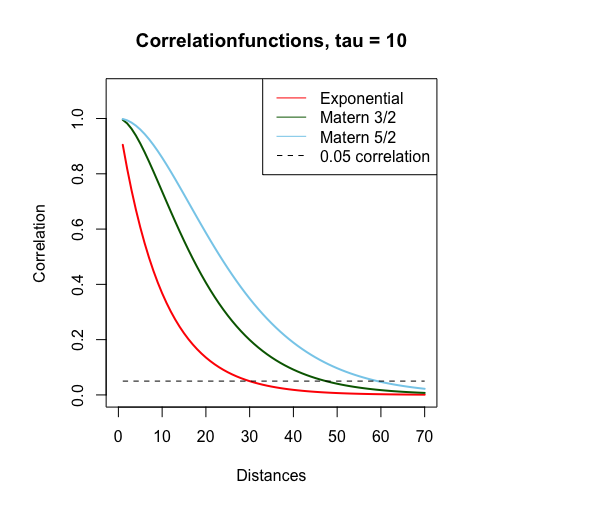
\includegraphics[width=1.3\linewidth]{figurer/correlation_tau10.png}
     \label{fig:data_original}
     \caption{Correlation with $\tau = 10$ as function of distance.}
   \end{minipage}
   \hspace{0.1pt}
   \begin{minipage}{0.475\textwidth}
     \centering
     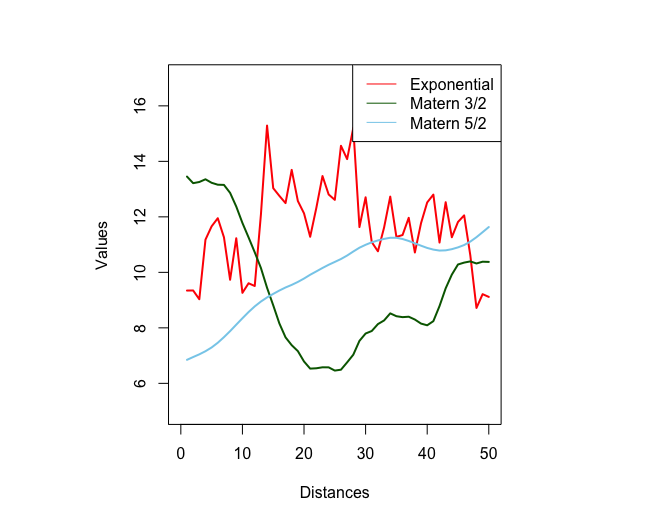
\includegraphics[width=1.3\linewidth]{figurer/sample_path-sigma10phi10.png}
	 \label{fig:data_original_reduced}
	 \caption{Sample path from model (\ref{model:hm}), $\sigma = 10$, $\phi = 10$.}
	 \end{minipage}
\end{figure}




\subsection{Gaussian processes} \label{sec:gaussian_processes}
Associated with every GRF is a underlying Gaussian process detailing the distributions of the variables contained in the field. The fundamental characterization of such a process is that all finitie-dimensional joint distributions for the variables of the process is multivariate normally distributed (MVN), and especially that each variable is normally distributed. Being distributed as a MVN, a Gaussian process is completely determined by its mean and covariance functions \textbf{ref til linstatbok}. Thus, the mean and covariance functions of a process are often a focus point in dealing with a Gaussian process. \\

Amongst the many favourable properties of MVN distributions, we also have that the best predictor for an unobserved variable in a Gaussian process is linear function of the observed variables. The predictor being a linear function of MVN distributed variables, the predictor as well is MVN distributed with an adjusted mean and covariance. \\ 

More precisely, if $\begin{bmatrix} A \\ B \end{bmatrix}$ is a vector of $n$ stochastic variables associated with a Gaussian process, meaning $\begin{bmatrix} A \\ B \end{bmatrix}$ has a distribution on the form of $\mathcal{MVN}(\begin{bmatrix} \mu_A \\ \mu_B \end{bmatrix}, \begin{bmatrix} \Sigma_{AA} & \Sigma_{AB} \\ \Sigma_{BA} & \Sigma_{BB} \end{bmatrix})$, where $\Sigma_{AB} = \Sigma_{BA}^T$ denotes the covariance between the variables in $A$ versus the variables in $B$.  given B, we have exact results for the best linear predictor. $P(A | B = b)$ will then be $MVN$, with corrected mean $\mu_{A | B}$ and variance $\Sigma_{A | B}$ as:
\begin{align}
\mu_{A | B} &= \mu_A + \Sigma_{AB}\cdot \Sigma_{BB}^{-1}\big( b - \mu_B \big) \label{eq:gaussian_conditional_expectancy} \\
\Sigma_{A | B} &= \Sigma_{AA} - \Sigma_{AB} \cdot \Sigma_{BB}^{-1} \cdot \Sigma_{BA} \label{eq:gaussian_conditional_variance}
\end{align}

In an uformal setting, one may interpret this as a linear smoothing of the parameters for the MVN distribution of $A$. Especially it's worth noting that since the covariance matrix $\Sigma_{BB}$ is positive definite, its inverse is as well, meaning that the diagonal entries of $\Sigma_{AB} \cdot \Sigma_{BB}^{-1} \cdot \Sigma_{BA}$ are all greater or equal to zero. As the variance of $P(A | B = b)$ are the diagonal elements of $\Sigma_{A|B}$, we have that the elementwise variance after conditioning on $B$ is lower or equal than with no conditioning: 
\begin{equation}
\Sigma_{A|B} = \Sigma_{AA} - \Sigma_{AB} \cdot \Sigma_{BB}^{-1} \cdot \Sigma_{BA}
\implies \Sigma_{A|B}[i, \ i]  \leq \Sigma_{AA}[i, \ i] \quad  i = 1, \dotsc, n.
\end{equation}
where $\Sigma_{AA}[i, \ i]$ denotes the entry at index $(i, i)$ in the matrix.
The equality will only hold for $\Sigma_{AB} = \mathbf{0}$, which would mean that $Cov(A, B) = 0$. Intuitively, this makes sense as then the variables of $B$ have no relation to the variables in $A$. \\

Evidently from the aforementioned property, when dealing with a Gaussian process it would be favourable to have well-defined expressions for its mean and covariance. One possible solution in the case of the process-covariance is to use a covariance function to define the covariance between variables given some criteria to evaluate.

\textbf{Model and specify the model that's been used}

\begin{figure}[!htb]
	%\hspace*{\fill}     
   \begin{minipage}{0.475\textwidth}
     \centering
     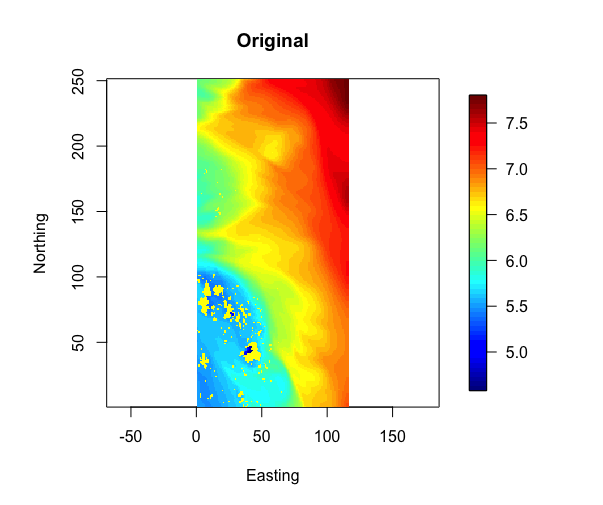
\includegraphics[width=1.25\linewidth]{figurer/original.png}
        \caption{Original termperaturedata}
        \label{fig:data_original}
   \end{minipage}
   \begin {minipage}{0.44\textwidth}
     \centering
     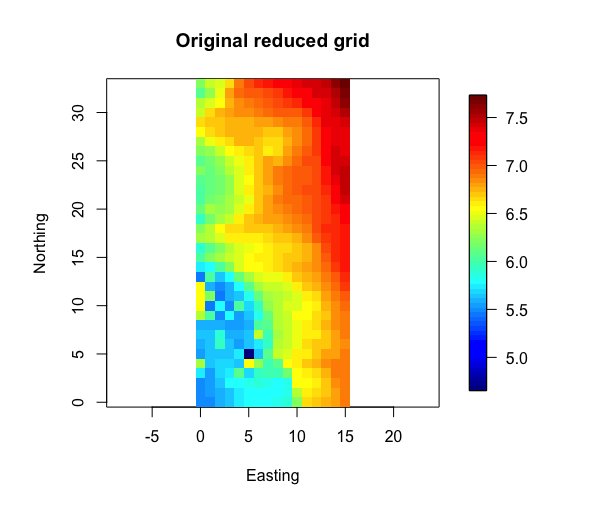
\includegraphics[width=1.3\linewidth]{figurer/original_reduced.png}
     \caption{The original data interpolated to a reduced grid for use in prediction}
	 \label{fig:data_original_reduced}
   \end{minipage}
\end{figure}

\subsection{Model design} \label{model:hm}
One common way of defining the model used to relate the process of data acquisition to the properties of the GRF is by a hierarchical model. A hierarchical model divides the spatial design model 
into three parts: 
\begin{itemize}
\item Data model - Describes the relation between process and datasampling
\item Process model - Describes the model properties of the GRF 
\item Prior model - Priors used in the case of Bayesian modelling of parameters
\end{itemize}

An example of such a model may be given for the case example used to generate the sample paths in \textbf{Ref til sample paths eksempel} \ref{fig:sample_paths}. In this model the parameters of the underlying GP is fixed, so 'Prior model' is omitted. Denoting $Z$ as the sampled data, $Y$ as the underlying GP and parameters $\mu, \tau, \sigma^2, \phi$:
\begin{itemize}
\item Data model: $Z(\vec{s}) \sim \mathcal{N}\big(F(\vec{s}) \cdot Y, \ \phi^2I(\vec{s})\big)$
\item Process model: $Y \sim \mathcal{N}\big( \vec{\mu}, \ C_Y(D, \sigma^2, \tau) \big)$ 
\end{itemize}
where $\vec{s} \in \mathcal{R}^n \times \mathcal{R}^2$ is the matrix of coordinates for the points in question, $D$ denotes a symmetric $n \times n$ matrix of distances between the points in the field, F is a matrix indicating sampling of data and $C_Y(\dots)$ the chosen covariance function. For the sample path examples in \ref{fig:sample_paths} the three covariance functions in \ref{eq:covariance_functions} have been used. \\

By using the linearity property of Gaussian variables, we may write the models as linear combinations of their means and covariances, i.e. 
\begin{itemize}
\item Data model: $Z(\vec{s}) = F(\vec{s}) \cdot Y + \epsilon, \quad \epsilon \sim \mathcal{N} \big(\vec{0},\phi^2I(\vec{s}) \big)$
\item Process model: $Y = \vec{\mu} + \rho, \quad \rho \sim \mathcal{N} \big(\vec{0}, \ C_Y(D, \sigma^2, \tau ) \big) $ 
\end{itemize}
This is a unique property of models with a GRF and Gaussian distributed errors and is of no difference compared to the first model.

\textbf{Specify the model here}

\subsubsection{GLS}
The trendfunction is another matter. As we are unaware of any data in the grid that may be related to the trend of the GRF model, the better option that is left is to estimate the trend based on the datacollection. The trendfunction is defined as a polynomial function of spatial location on the form $\mu(\vec{s}) = X(\vec{s})\vec{\beta}$, where X is a design matrix corresponding to the locations $\vec{s}$ and $\vec{\beta}$ is vector of coefficients. By doing so we may utilize results from the theory of \textit{Generalized Least Squares} (GLS) in the estimation of trend. One particular advantage of using GLM is that we are guaranteed by the Gauss-Markov Theorem that the GLR estimates is the \textit{Best Linear Unbiased Estimator} (BLUE) for the vector of coefficients $\vec{\beta}$. \\

One of two caveats with using GLR estimates is that one still need to specify the polynomial trendfunction to fit the data, meaning there's still a selection process. As the trendfunction is to specified by spatial location for this case, one must face the second caveat. The GLR estimates are the BLUE only for the data and their associated spatial location used in the estimation, giving no guarantee for the prediction of data not part of the estimates. By this, the trendfunction will be selected to be a polynomial of lower order with simple interaction between easting- and northing-coordinates. This has been chosen as an prediction far away from the sample data will typically be over- or underpredicted by an unacceptable amount using a higher-order polynomial. This is due to the covariates of said polynomial will be fitted to the data that has been sampled, which in this case will be done mainly by specified design of low regularity. In sampling designs with high regularity over the field, this is effect is handled as then the estimation will try to adapt to grid points that are within a certain distance from each other. An example of this issue is shown in figures \ref{fig:predictions_polynomials} along with the original data for comparison.  \\

When the samples are drawn from a distribution with known correlation matrix $\Omega = \sigma^2 \cdot W$, with $\sigma^2$ is constant finite variance parameter and $W$ the correlation matrix, the estimates of $\vec{\beta}$ converge in distribution to a MVN, or more precisely
\begin{equation}
\hat{\vec{\beta}} \xrightarrow[]{d} \mathcal{MVN} \big( \ \vec{\beta}, \ (X^T \Omega^{-1} X)^{-1} \big)
\end{equation}
where $X$ denotes the associated design matrix of the samples estimated.


\begin{figure}[!htb]
	%\hspace*{\fill}     
   \begin{minipage}{0.475\textwidth}
     \centering
     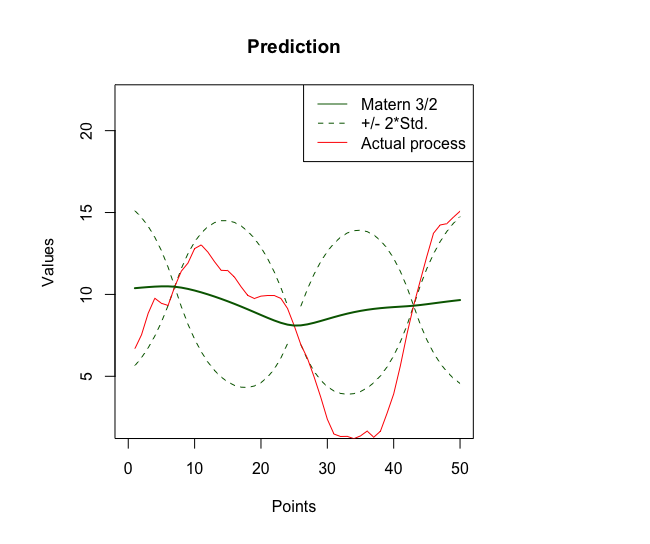
\includegraphics[width=1.25\linewidth]{figurer/prediction_325.png}
        \caption{Original termperaturedata}
        \label{fig:data_original}
   \end{minipage}
   \begin {minipage}{0.44\textwidth}
     \centering
     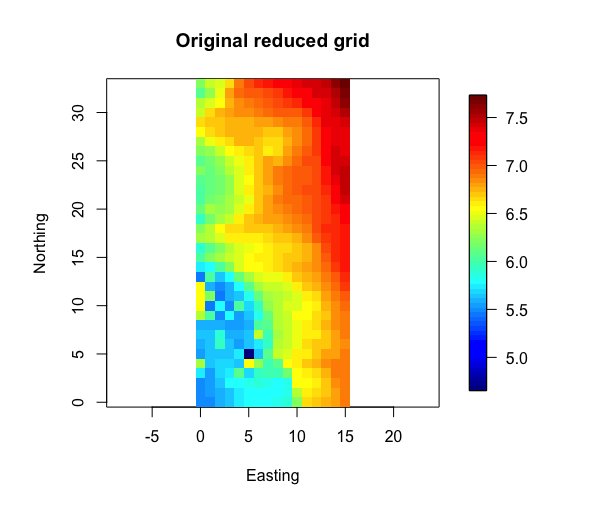
\includegraphics[width=1.3\linewidth]{figurer/original_reduced.png}
     \caption{The original data interpolated to a reduced grid for use in prediction}
	 \label{fig:data_original_reduced}
   \end{minipage}
\end{figure}

\subsubsection{Deriving the posterior GRF}
The ultimate goal of the analysis is to provide a result for the posterior distribution of the underlying Gaussian process, given some sample data, that is $P \big( Y(\vec{s}) | Z(\vec{s_0}) \big)$ where $\vec{s}$ denotes the whole coordinates of the whole field and $\vec{s_0}$ denotes the coordinates of samples obtained. This distribution is derived as 
\begin{align*}
\begin{split}
P \big( Y(\vec{s}) | Z(\vec{s_0}) \big) &= \int \int P \big( Y(\vec{s}), \sigma^2, \tau | \ Z(\vec{s_0}) \big) \ d\sigma^2 \ d\tau \\
&= \int \int P \big( Y(\vec{s}) | Z(\vec{s_0}), \sigma^2, \tau \big) \cdot P\big( \sigma^2, \tau | Z(\vec{s_0}) \big) \ d\sigma^2 \ d\tau 
\end{split}
\end{align*}
Further, we use Bayes Theorem 
\begin{align}\label{eq:posterior_prior}
\begin{split}
P\big( \sigma^2, \tau | Z(\vec{s_0}) \big) &\propto P\big( Z(\vec{s_0}) | \sigma^2, \tau \big) \cdot P\big( \sigma^2, \tau \big) \\[5pt]
&\propto P\big( Z(\vec{s_0}) | \sigma^2, \tau \big) \cdot P\big( \sigma^2 \big) \cdot P\big( \tau \big) \\[10pt]
\implies P\big( \sigma^2, \tau | Z(\vec{s_0}) \big) &= \frac{P\big( Z(\vec{s_0}) | \sigma^2, \tau \big) \cdot P\big( \sigma^2 \big) \cdot P\big( \tau \big)}{\int \int P\big( Z(\vec{s_0}) | \sigma^2, \tau \big) \cdot P\big( \sigma^2 \big) \cdot P\big( \tau \big) d\sigma^2 d\tau}
\end{split}
\end{align}
This implies that 
\begin{equation}\label{eq:grf_posterior}
\hspace*{-0.1cm}
P \big( Y(\vec{s}) | Z(\vec{s_0}) \big) = \int \int P \big( Y(\vec{s}) | Z(\vec{s_0}), \sigma^2, \tau \big) \cdot \frac{P\big( Z(\vec{s_0}) | \sigma^2, \tau \big) \cdot P\big( \sigma^2 \big) \cdot P\big( \tau \big)}{\int \int P\big( Z(\vec{s_0}) | \sigma^2, \tau \big) \cdot P\big( \sigma^2 \big) \cdot P\big( \tau \big) d\sigma^2 d\tau} \ d\sigma^2 \ d\tau
\end{equation}

An exact analytical result for the posterior found in both \ref{eq:posterior_prior} and \ref{eq:grf_posterior} may be found under the with the appropriate priors, but to acommodate any type of prior from a probability distribution, the integrals is approximated by a simple numerical procedure. This is done by discretizing the domain of $\sigma^2$ and $\tau$ and summing over the discretizied values with some weight $\Delta$ for each discretization to ensure normalization, giving an approximation as
\begin{align*}
\begin{split}
P \big( Y(\vec{s}) | Z(\vec{s_0}) \big) &\approx \frac{1}{\Pi}\sum_{\tau_i}^{n_{\tau}} \sum_{\sigma^2_j}^{n_{\sigma}} P \big( Y(\vec{s}) | Z(\vec{s_0}), \sigma^2_j, \tau_i \big) \cdot P\big( Z(\vec{s_0}) | \sigma^2_j, \tau_i \big) \cdot P\big( \sigma^2_j \big) \cdot P\big( \tau_i \big) \cdot \Delta_{ij}
\end{split}
\end{align*}
With $\Pi = \sum_{\tau_i}^{n_{\tau}} \sum_{\sigma^2_j}^{n_{\sigma}} P\big( Z(\vec{s_0}) | \sigma^2_j, \tau_i \big) \cdot P\big( \sigma^2_j \big) \cdot P\big( \tau_i \big) \cdot \Delta_{ij}$ as the normalizing constant. \\

For this integration to be performed, four distributions need to be defined: $P\big( \sigma^2_j \big)$ and $P\big( \tau_i \big)$ are priors given by the model, $P\big( Z(\vec{s_0}) | \sigma^2_j, \tau_i \big)$ is known MVN by the model specification and lastly we have that $P \big( Y(\vec{s}) | Z(\vec{s_0}), \sigma^2_j, \tau_i \big)$ is MVN by the results presented in \ref{sec:gaussian_processes} with $Y(\vec{s})$ as $A$ and $Z(\vec{s_0})$ as $B$. \\

When performing the numerical integration, it is noted that it's the mean and variance of $P\big( \sigma^2, \tau | Z(\vec{s_0}) \big)$ that's of relevance for the predictions. By similar arguments as above, one gets:
\begin{align}\label{eq:expected_variance_grf_posterior}
\begin{split}
\mathbf{E} \big( Y(\vec{s}) | Z(\vec{s_0}) \big) &= \int \int \mathbf{E} \big( Y(\vec{s}) | Z(\vec{s_0}), \sigma^2, \tau \big) \cdot \frac{P\big( Z(\vec{s_0}) | \sigma^2, \tau \big) \cdot P\big( \sigma^2 \big) \cdot P\big( \tau \big)}{\int \int P\big( Z(\vec{s_0}) | \sigma^2, \tau \big) \cdot P\big( \sigma^2 \big) \cdot P\big( \tau \big) d\sigma^2 d\tau} \ d\sigma^2 \ d\tau \\
&\approx \frac{1}{\Pi}\sum_{\tau_i}^{n_{\tau}} \sum_{\sigma^2_j}^{n_{\sigma}} \Delta_{ij} \cdot \mathbf{E} \big( Y(\vec{s}) | Z(\vec{s_0}), \sigma^2_j, \tau_i \big) \cdot P\big( Z(\vec{s_0}) | \sigma^2_j, \tau_i \big) \cdot P\big( \sigma^2_j \big) \cdot P\big( \tau_i \big) \\
\mathbf{Var} \big( Y(\vec{s}) | Z(\vec{s_0}) \big) &= \int \int \mathbf{Var} \big( Y(\vec{s}) | Z(\vec{s_0}), \sigma^2, \tau \big) \cdot \frac{P\big( Z(\vec{s_0}) | \sigma^2, \tau \big) \cdot P\big( \sigma^2 \big) \cdot P\big( \tau \big)}{\int \int P\big( Z(\vec{s_0}) | \sigma^2, \tau \big) \cdot P\big( \sigma^2 \big) \cdot P\big( \tau \big) d\sigma^2 d\tau} \ d\sigma^2 \ d\tau \\
&\approx \frac{1}{\Pi}\sum_{\tau_i}^{n_{\tau}} \sum_{\sigma_j^2}^{n_{\sigma}} \Delta_{ij} \cdot \mathbf{Var} \big( Y(\vec{s}) | Z(\vec{s_0}), \sigma^2_j, \tau_i \big) \cdot P\big( Z(\vec{s_0}) | \sigma^2_j, \tau_i \big) \cdot P\big( \sigma^2_j \big) \cdot P\big( \tau_i \big) \\\end{split}
\end{align}
with $\Pi$ defined as before. The expressions of $\mathbf{E} \big( Y(\vec{s}) | Z(\vec{s_0}), \sigma^2, \tau \big)$ and $\mathbf{Var} \big( Y(\vec{s}) | Z(\vec{s_0}), \sigma^2, \tau \big)$ is given in \ref{eq:gaussian_conditional_expectancy} and \ref{eq:gaussian_conditional_variance}.

\textbf{
Figurer
\begin{itemize}
\item cov func
\item realisasjon GRF
\item conditional grf (fix par, høy / lav korrelasjon)
\end{itemize} 
fyre inn hierarkisk modell
4.2.2-3 her
}

\newpage
\section{Spatial Design}
\subsection{Sampling design} 
\label{sec:sampling_design}
In spatial prediction, the choice of which spatial locations, or spatial design, to sample data from becomes critical. In the model setting, this means defining how our matrix $F(\vec{s})$ mentioned in (\ref{}) is constructed. In order to achieve the best design, one would have to choose in cohesion with the model that is defined for the data situation and as to what criteria the model is trying to satisfy. 

There are two common situations when producing sampling designs. Firstly we have the \textit{retrospective design}, where one assesses the sampling design after obtaining information about the attributes of interest. A goal in this setting might be to reduce the number of sampling locations without a significant loss in the amount or quality of information. This problem is exemplified by a want to economize measuring-stations while still achieving satisfactory measurements from the remaining locations.  

The second approach is that of \textit{proactive design}. In this form, the overall goal is to design a set of sampling locations in advance of the data acquisitioning that align with some criteria set for the project. The criteria is most often set on a applicationbased setting, indicating that it doesn't exist any general solution to produce the optimal design. Typically in a predictive setting, criterias that revolve around minimizing the variance or predicitve error of a design or maximizing the entropy is common. Two examples of criterias relating to the variance are found in equations (\ref{eq:criteria_binney}) and (\ref{eq:criteria_diggle}). 


The setting in which this criteria was used was the desire to find the optimal path through a graph that were modelled as a random field \cite{BinneyEtAl}. The criteria was to minimize the \textit{Expected Mean Squared Error} (EMSE), that they calculated as 
\begin{equation} \label{eq:criteria_binney}
\text{EMSE} = \frac{1}{n} [tr(\Sigma_p) - tr(\Sigma_o)]
\end{equation}
where $\Sigma_p$ denotes the posterior covariancematrix and $\Sigma_o$ denotes the prior covariancematrix.

For equation (\ref{eq:criteria_diggle}), the setting was retroactive design planning, were the ultimate goal was to remove as many measurement-locations in a random field without significant loss in measurement amount or quality \cite{DiggleEtAl}. This criteria was adhered to by minimizing the equation 
\begin{equation} \label{eq:criteria_diggle}
E(\vec{\nu}) = \int_A E_{Y|\theta_0} [Var(S(x)|Y)]dx
\end{equation}
where $S(x)$ denotes a function of the proposed reduced sampling design, $Y$ known data and $\theta_0$ the true parameter values.

To adhere to the criteria that's set, the design need not be solved within the workframe as stated by the model ones uses. Diggle \& Lophaven \cite{DiggleEtAl} refers to some purely geometrical approaches that may work well for finding adequate designs. In this project a satisfiable design will be estimated on the basis of a combination of predefined design proposals, i.e. the project will use focus on proactive design. The criteria that will be used in this project is minimizing the spatially averaged standard deviation of the proposed sample design, i.e. 
\begin{equation} \label{eq:criteria}
I = \sum_{Z_a} \sum_{i=1}^n \sqrt{ Var (Y_i | Z_a, Z) } P(Z_a | Z) .
\end{equation}
where $Z_a$ denotes the proposed design, $Z$ current data that has been acquired and $Y_i$ as the latent process at the location to be predicted. 

\subsection{Constructing designs in Bayesian hierarchical models}

med usikkerhet så må man midle over parameterene for begge fordelingene, både varians. -> pseudokode

\newpage
\section{Case}
\subsection{Case introduction}
\subsubsection{Introduction and case specification} \label{subsub:goals}
In this case I've been presented with the task of performing a predictive analysis of an attribute that may be modelled by a random field. The scenario is that there is a desire in knowing the temperature for a specific physical location, and one would like to perform predictive analysis with the following goals in mind:
\begin{itemize} 
\item Perform satisfactory accurate predictions
\item Minimize data acquirement needed
\end{itemize} 
In order to ensure that these goals will be met, the analysis of the case will be set up within the framework of a hierarchical model as described in (\ref{hm:linear_model}). Within this setting, suitable criterias must be set so that the analysis may be performed in a way that easily relates to these goals. The criterias set for this case will be to minimize equation (\ref{eq:criteria}) where the proposed paths focus on covering areas where the prediction variance is high. Informally we may say that we are seeking for the most uncertainty-reducing paths of data sampling. 

\subsubsection{Input}
The only information that we're presented with beforehand is a variogram computed on the basis of simulation model output based on weather forecasts, oceanographic models and satelite data. This is however reckoned as slightly unreliable data and must be handled accordingly. The area in which the analysis will be based on is given as a list of xy-coordinates with each coordinate being given a z-variable denoting the numerical value to the attribute of interest. There is a total of 29116 coordinates, ordered into a rectangular grid with size 116 in x-direction and size 251 in y-direction. The directions will informally be called easting and northing when plotting. The variogram is presented in (\ref{fig:variogram}) along with the original data which we desire to predict. 

\begin{figure}[p]
\minipage{0.45\textwidth}
	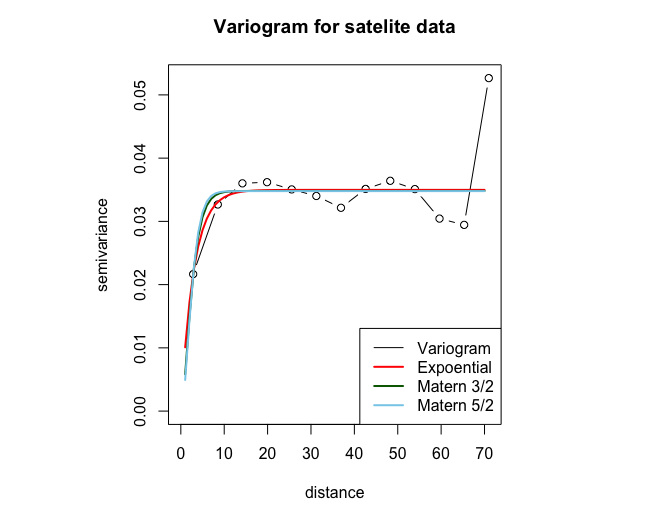
\includegraphics[width=1.4\linewidth]{figurer/variogram_covariancefunctions.png}
    \caption{Variogram given as input to the case.}
    \label{fig:variogram}
	\endminipage\hfill
	\minipage{0.45\textwidth}
  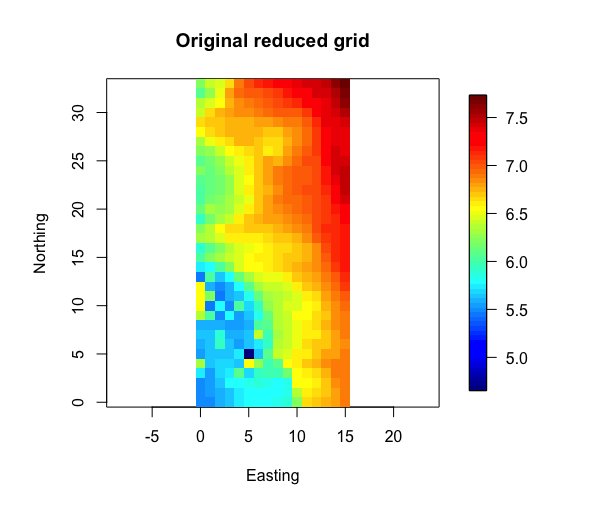
\includegraphics[width=1.4\linewidth]{figurer/original_reduced.png}
   \label{fig:original_data}
	 \caption{Actual data that are to be predicted on a reduced grid from the original.}
\endminipage
\end{figure}

\begin{figure}[p] 
\minipage{0.5\textwidth}
	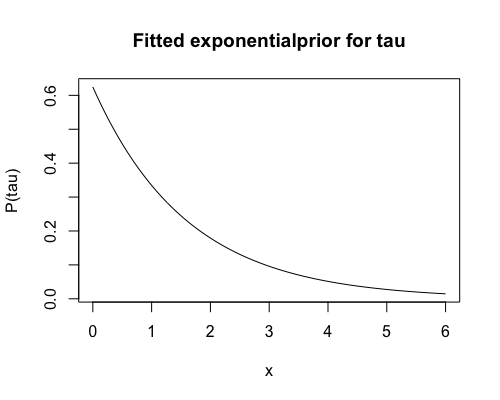
\includegraphics[width=1\linewidth]{figurer/fitted_exponential.png}
     \caption{Fitted prior distribution for $\tau$.}
     \label{fittedexponential}
	\endminipage\hfill
	\minipage{0.5\textwidth}
  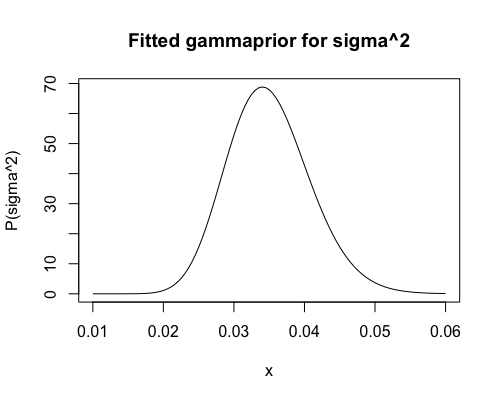
\includegraphics[width=1\linewidth]{figurer/fitted_gamma.png}
	 \caption{Fitted prior distribution for $\sigma^2$}
	 \label{fittedgamma}
\endminipage
\end{figure}

\subsubsection{Model specification and starting point of analysis} \label{subs:model}
As a necessary preliminary for the predictive analysis the temperature attribute of all the coordinates is modelled as a stochastic variable. Attaining a Gaussian process to describe trend and variability of model, the grid is viewed as a GRF. The connection between variables in this model will revolve around spatial location within the grid, where the trendfunction will be estimated by GLS regression on the sampled data. The covariance will be described by an isotropic, where results from all three covariancefunctions of (\ref{eq:covariance_functions}) will be presented individually. \\
The model process is fitted into the hierarchical model (HM) design described in (\ref{model:hm}). With $Y$ denoting the temperature variables at locations $\vec{s}$, that's set to be distributed according to the Gaussian process, the hierarchical model follows as
\begin{align*}
\begin{split}
\textbf{Data model: }& \vec{Z}(\vec{s}) = \vec{Y}(\vec{s}) + \vec{\epsilon}(\vec{s}), \quad \vec{\epsilon}(\vec{s}) \sim \mathcal{MVN} \big(\vec{0},\phi^2I(\vec{s}) \big) \\
\textbf{Process model: }& \vec{Y} = \vec{\mu} + \rho(\vec{s}), \quad \rho(\vec{s}) \sim \mathcal{MVN} \big(\vec{0}, \ C_Y(D(\vec{s}), \sigma^2, \tau ) \big) \\
\textbf{Prior model: }& \sigma^2 \sim \text{Gamma}(\alpha, \kappa), \quad \tau \sim \text{Exp}(\lambda)
\end{split}
\end{align*}
The intensity of the sampling noise, $\phi^2$, is the only one of the parameters that will be fixed. The motivation for doing so is that sampling noise may be viewed as more related to the equipment being used than the analysis in which it is included. Compared to the other parameters, one may have much more information about this parameter, as it may be stated by the equipment manufacturer or be tested separately in controlled environments. For the results, $\phi^2 = 0.2$ has been used. 

With the trend $\vec{\mu}$ is to be estimated by GLS on the sampled data eventually the data model is redefined as 
\begin{align} \label{eq:data_model}
\begin{split}
\textbf{Data model: }\vec{Z}(\vec{s}) &= X(\vec{s})\hat{\vec{\beta}} + \epsilon(\vec{s}) + \rho(\vec{s}) \\
\implies \vec{Z}(\vec{s}) &\sim \mathcal{MVN} \big( X(\vec{s})\hat{\vec{\beta}}, \ X(\vec{s}) \Sigma_{\hat{\beta}} X(\vec{s})^{T} + C_Y(D(\vec{s}), \sigma^2, \tau ) + \phi^2I(\vec{s}) \big)
\end{split}
\end{align}
where  Var${\hat{\beta}} = \Sigma_{\hat{\beta}} =  \bigg( X(\vec{s_0})^T \cdot \big( C_Y(D(\vec{s_0}), \sigma^2, \tau \big) + \phi^2I(\vec{s_0}) )^{-1} \cdot X(\vec{s_0}) \bigg)^{-1}$. \\

\subsection{Analysis}
\subsubsection{Choosing prior-parameters}
As a consequence of defining our model with prior-distributions for $\sigma^2$ and $\tau$, we must somehow estimate or choose parameters for their distributions. In order to do so, the variogram given as a part of the case preliminary has been utilized to estimate the GRF parameters of $\sigma^2$ and $\tau$. Given the three covariancefunctions in \ref{eq:covariance_functions}, the one may try to fit the the parameters of the chosen covariancefunction to the line. Denoting the discrete variogram values at points $k$ as $\gamma_k$ and the fitted covariancefunction at the same points as $\hat{\gamma}_k(\sigma^2, \tau)$, this is done by minimizing the associated lossfunction
\begin{equation}
Loss(\sigma^2, \tau) = \sum_k \bigg( \frac{\gamma_k - \hat{\gamma}_k(\sigma^2, \tau)}{\gamma_k} \bigg)^2
\end{equation}
Notice that we only have two parameters to be estimated for each covariancefunction as the nugget effect has been assumed to be negligible, resulting in more stable computation of fit. This minimization has been performed using the \textit{variofit} function in the \textit{geoR} package found in the programming environement R. Obviously, the covariance functions are exponentially decaying as a function of distance with the three chosen in \ref{eq:covariance_functions}. In order to visually compare the fit, we use the relation between the variogram of a isotropic process and its covariancefunction that is
\begin{align} \label{eq:variogram_covariancefunction}
\begin{split}
    2\gamma(\textbf{s},\textbf{t}) &= Var(Y(\textbf{s}) - Y(\textbf{t})) \\
    &= Var(Y(\textbf{s})) + Var(Y(\textbf{t})) - 2Cov(Y(\textbf{s}),Y(\textbf{t})) \\
    \implies \gamma(\textbf{s},\textbf{t}) &= \sigma^2 - Cov(\|\textbf{s}-\textbf{t}\|)
\end{split}
\end{align}

The variogram is then overlain with fitted covariancefunctions, adapted by equation (\ref{eq:variogram_covariancefunction}), from \ref{eq:covariance_functions} in figure (\ref{fig:variogram}).  

Denoting the estimated values as $\hat{\sigma}^2$ and $\hat{\tau}$, one could have performed predictioning straight away. However, in an attempt to reduce the uncertainty in using this variogram, $\hat{\sigma}^2$ and $\hat{\tau}$ is used to fit parameters for the priors. This has been done by using a \textit{method of moments} inspired approach. As we have a single parameter prior for $\tau$, its mean and variance is estimated by 
\begin{align}
\hat{\lambda} = \frac{1}{\hat{\tau}}
\end{align}
With $\sigma^2$ given a gamma-prior, one needs to estimate two parameters. Denoting $\sum_k (\gamma_k - \hat{\sigma}^2)^2$ as $s_*^2$, the following approximation is used to set parameters $\alpha$ and $\beta$:
\begin{align}
\mathbf{E}(\sigma^2) = \frac{\alpha}{\beta} \approx \hat{\sigma}^2, \quad
\mathbf{Var}(\sigma^2) = \frac{\alpha}{\beta^2} \approx s_*^2 
\implies 
\hat{\alpha} = \frac{(\hat{\sigma}^2)^2}{s_*^2}, \quad  \hat{\beta} = \frac{\hat{\sigma}^2}{s_*^2}
\end{align}

The resulting prior-distributions are presented in figures (\ref{fittedexponential}) and (\ref{fittedgamma}).

\subsubsection{Discretizing the prior domains}
As the analysis relies on a numerical summation over the prior domains, a strategy must be defined to discretize the domains into $n_{\sigma^2}$ and $n_{\tau}$ divisions used the summation \ref{eq:expected_variance_grf_posterior}. In this case a method of \textit{stratified sampling} has been used. Given size-input $n_{\sigma^2}$, $(0,\inf)$ is subdivided into $n_{\sigma^2}$ divisions, each part corresponding to a $\frac{1}{n_{\sigma^2}}$ probability mass of the prior. Random samples are simulated until minimum one sample within each division is obtained. The same procedure is performed for $n_{\tau}$. 

The joined domain of $\tau$ and $\sigma^2$ is then considered a grid, with each cell corresponding to samples $(\tau_i, \sigma_j^2)$ having a probability mass of $\Delta_{ij} = \frac{1}{n_{\sigma^2} \cdot n_{\tau}}$ due to independence of priors. With both the normalizing constaHowever, may also be definedt and the summation for predictioThis progame discretization, all $\Delta_{ij}$ cancels as they are independent of $(\tau_i, \sigma_j^2)$ and are therefore omitted from the calculations. A disadvantage is obviously the problem of simulating random samples for all the divisions if the number of divisions become high. However, $n_{\tau}$ and $n_{\sigma^2}$ is kept relatively low in this case. 

\subsubsection{Results}	
Due to time-limitations, only a select predefined designs were used to produce results. The designs are presented in figure (\ref{fig:designs}). 

As the model is reliant on estimation of trend, an initial data sample has to be obtained. To estimate the spatially averaged predictive standard deviation, each design presented in figure (\ref{fig:designs}) was used as an initial design. Samples was obtained from this initial design, and possible new designs for further predictive analysis of the area was the remaining sample designs. Using the procedure described in subsection (\ref{}), results are presented in the table below. Each number signifies the estimated spatially averaged standard deviation of using samples $Z$ from the design at the top of the table as the initial sample, with the design  on the left as the next path $Z_a$. 
\\

\hspace{-25pt}
\begin{tabular}{ l || c | c | c | c | c | c | c | c } 
\label{tab:bayes_predictive_variance}
$Z_a$ \textbackslash  $Z$ & Design 1 & Design 2 & Design 3 & Design 4 & Design 5 & Design 6 & Design 7 & Design 8 \\
\hline \hline
Design 1 & - & 548.0111 & 490.2626 & 472.2716 & \textbf{465.4389} & \textbf{461.4315} & \textbf{458.3172} & \textbf{457.1136} \\
Design 2 & 548.0420 & - & 549.6023 & 490.1057 & 473.6499 & 465.6733 & 460.4351 & 458.5897 \\
Design 3 & 490.2403 & 549.4966 & - & 547.7782 & 495.0345 & 474.8508 & 464.7677 & 461.2044 \\
Design 4 & 472.3915 & 490.0712 & 547.8146 & - & 580.9237 & 498.8230 & 473.9019 & 466.1729 \\
Design 5 & 465.5245 & 473.6227 & 495.0963 & 580.9661 & - & 573.4793 & 495.3815 & 476.5188 \\
Design 6 & 461.4052 & 465.4790 & 474.7950 & 498.7048 & 573.4010 & - & 555.6704 & 495.8328 \\
Design 7 & 458.3496 & 460.5030 & 464.8691 & 473.9674 & 495.4149 & 555.7863 & - & 559.4372 \\
Design 8 & \textbf{457.1382} & \textbf{458.4126} & \textbf{461.1775} & \textbf{466.1601} & 476.5174 & 495.9166 & 559.3891 & -
\end{tabular}

\begin{figure}[p]
	\hspace{-55pt}
	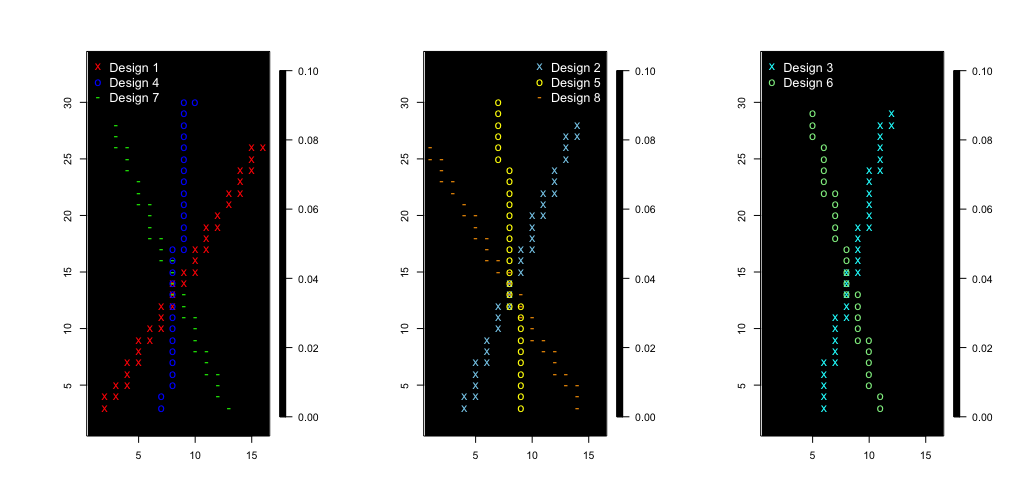
\includegraphics[width=1.25\linewidth]{figurer/design_lines.png}
    \caption{Sampling designs used to produce results.}
    \label{fig:designs}
\end{figure}
\newpage

\section{Conclusion}
\textbf{Summer opp} \\
\textbf{Alternativer - komputasjonsmessig kostbart å bruke normalfordeling} \\


%\section{Conclusion}
%\textbf{Summer opp} \\
%\textbf{Alternativer - komputasjonsmessig kostbart å bruke normalfordeling} \\

\newpage
\begin{thebibliography}{9}
\addcontentsline{toc}{section}{References}

\bibitem{EidsvikEtAl} Eidsvik, Jo and Mukerji, Tapan \& Bhattacharjya, Debarun (2015) \\ \emph{Value of Information in the Earth Sciences - Integrating Spatial Modeling and Decision Analysis}, \\ Cambridge University Press, 2015. 

\bibitem{RasmussenEtAl} Rasmussen, C. E. \& Williams, C. K. I. \\ \emph{Gaussian Processes for Machine Learning}, \\ the MIT Press, 2006.

\bibitem{DiggleEtAl}Diggle, Peter \& Lophaven, Søren \\ \emph{Bayesian Geostatistical Design}, \\ Scandinavian Journal of Statistics, volume 33 (2006): 53-64, print.

\bibitem{CressieEtAl} Cressie, Noel \& Wikle, Christopher K. \\ \emph{Statistics for Spatio-Temporal Data}, \\ John Wiley \& Sons (2011).

\bibitem{LeEtAl} Le, Nhu D. \& Zidek, James V. \\ \emph{Statistical Analysis of Environmental Space-Time Processes}, \\ Springer Science+Business Media Inc. (2006).

\bibitem{BinneyEtAl} Binney, Jonathan \& Krause, Andreas \& Sukhatme, Gaurav S. \\ \emph{Optimizing waypoints for monitoring spatiotemporal phenomena}, \\ The International Journal of Robotics Research (2013), print.

 %Use \cite{EidsvikEtAl} to refer in the text

\end{thebibliography}
\end{document}
